\section{Comparison with D-TDIBC}

The work of \cite{douasbin2018DelayedtimeDomainImpedance} provides a similar one-dimensional model for outflow acoustics based on their associated time delay by means of an impedance boundary called delayed time-domain impedance boundary conditions (D-TDIBCs). The method itself is reviewed in \chap{ch:lit-review}; here we simply observe potential benefits and drawbacks of the ADCBC method against the D-TDIBC method. Most obviously, D-TDIBC offers and validates only an outflow boundary method where ADCBC provides arbitrary acoustic delays for any characteristic boundary -- although only inflows and outflows are practical and validated here. Also, boundary values in D-TDIBC are calculated from information in the previous time step, with no information stored about the acoustic region. Hence, it is not immediately possible to access and visualise the acoustics in this downstream region. By contrast, a method has been provided in the ADCBC case, where the sample queues are reinterpreted as upstream and downstream spatial data of acoustic $\cl{L}_{1/5}$ values. This comes at the cost of a much larger memory burden required by these queues which is placed only onto the boundary processors. This memory footprint is not present in D-TDIBC. In both methods a strongly one-dimensional flow is required at the boundary and only delay effects under linear acoustics are modelled, although the nonlinear effects of impedance are implicitly involved in the impedance boundary formulation of D-TDIBC. This can be extended to model arbitrary reactions downstream boundaries to different frequencies in the envelope of the reflection coefficient. By comparison, ADCBC allows for other boundary treatments to potentially be `tacked on' by adding further terms to $\cl{L}_{1/5}(t)$. This has the natural benefit that the method should be easily implementable into systems already using an NSCBC formulation for non-reflecting boundaries. However, this has the drawback that the method is entirely reliant on the effectiveness of the baseline non-reflection. In both methods minimal cost is paid per step to apply the boundary conditions, but in the case of D-TDIBC a pre-processing cost must be paid to model a given time-delay and reflection coefficient envelope. Since no inflow formulation is given in their case, the movement of the DNS region through the physical domain would not be physical by means of changing the outflow delay, as we do with ADCBC.




\section{Report Conclusions}

This report performed a review of thermoacoustic instability literature and CFD literature which is relevant to combustion and combustion instabilities. We then thoroughly derived the methods used in the SUNSET code, which is used in this report to perform fully compressible, combustion simulations. The Acoustic Delay Characteristic Boundary Conditions (ADCBCs) are then introduced to tackle the problem of expensive thermoacoustic simulations by introducing a new boundary scheme based off the Navier-Stokes Characteristic Boundary Conditions (NSCBCs) formulation. Using this method, we provided a low order model for acoustics which leave the simulation domain by simply delaying their reentry into the domain, thus simulating a truncated duct where only the flame and surrounding hydrodynamics are resolved. Code schematics were presented for the method with the primary caveat being the large memory burden placed onto the inflow and outflow processors, although this is permissible for systems using modern hardware. Inflow instabilities were found which result from the acoustic-DNS coupling and have been reduced by either changing the boundary discretisation or increasing the amplitude of tangential filtering at the boundary, which is undesirable for applications to higher Reynold's number flows. Simulations were performed using ADCBC inflows and outflows to validate the method can reconstruct an acoustic bump which leaves and reenters the domain as well as standing wave modes of the full acoustic region. These examples illustrated how visualisation can be made of the acoustic region in post-processing to observe the full state of the system and how errors in the interpolation of these samples may result in poor wave reconstruction which becomes irrelevant for longer physical domains. A further example was then given of a thermoacoustically unstable flame in a one metre long closed-open tube which would have been much more expensive to resolve, had ADCBC not been used. We found excellent reproduction of the tube's acoustic modes using this truncated model for flame which is stationary in the tube.




\section{Future Work}

More immediate work ought to be done to further validate the proposed ADCBC method from \chap{ch:delay-bcs}, including investigating the interpolation of $\cl{L}_{1/5}$ values and ensuring that acoustic energy does not trivially increase over long time periods without a flame. Having said that, the method provides a framework for multiple different thermoacoustic applications, particularly for those taking place in long tubes. Thermodiffusive and thermoacoustically unstable flames can already be modelled with the caveat that the rapidly changing flame speeds of thermodiffusive flames likely mean it will exit the DNS domain. To remedy this, dynamic inflow velocities are required which do not couple to the acoustics and counteract the mean flame speed. This is also useful for other, non-thermodiffusive flames which reach secondary instability since the flame speed changes drastically under this regime. Another typical test case and one which is used to test the D-TDIBC method in \cite{douasbin2018DelayedtimeDomainImpedance} is a flame in a strong counterflow, held in place by an adiabatic cylindrical flame holder. Comparisons to their calculated eigenmodes could be found by simulating the same model geometry whilst also providing mode shapes in the fictitious domain. ADCBC should also be easily applicable to flames passing through arrays of cylinders (or other porous geometries). Typically, this is expensive to model due to the task of fitting the discretisation to the complex body and the large scale disparity in thermoacoustics. Utilising the LABFM discretisation in the SUNSET code coupled to low-order ADCBC allows us to model this phenomena for the cost of discretising only the flame and its surrounding hydrodynamic region.

Furthermore, the use of characteristic boundaries allows us to freely impose incoming acoustics through the inflow, $\cl{L}_{5, \rm{imposed}}(t)$ and outflow, $\cl{L}_{1, \rm{imposed}}(t)$ on top of their existing values from the acoustic delay. By implementing an imposed e.g.\ sinusoidal forcing to model an upstream loudspeaker playing a pure tone, we can trigger secondary instabilities in a model version of \cite{searby1991ParametricAcousticInstability}. This would allow us to more efficiently investigate secondary instability modes and their flame structures. This could be potentially elaborated into three dimensions to try and recreate the wavenumber measurements of \cite{delfin2024DeterminationMethodMarkstein}. Turbulent flow can also be imposed through the VFCBC method established in \cite{guezennec2009AcousticallyNonreflectingReflecting} and an attempt could be made to implement this on top of the existing ADCBC method, as above. Turbulent characteristic outflows would also need to be implemented for compatibility. This may allow us to simulate faster flows in broader domains which are expected to be turbulent, as well as potentially allowing us to observe the self-turbulent flames seen resulting from secondary instability in \cite{searby1992AcousticInstabilityPremixed}.

Thus far, we have gotten away with values of $\abs{R_{\rm{U}/\rm{D}}} = 1$, but more realistic boundaries have impedances which vary with frequency. Could this be explored using some predefined spectral filtering on the delayed $\cl{L}_{1/5}$ values? Practically speaking, a low-pass filter could be used to remove high-frequency noise and improve the quality of observed low frequency modes (at the cost of precluding high-frequency ones). More generally, the nonlinear acoustic effects which are not being modelled here could be included by coupling an acoustic solver to the DNS inflow and outflow. Using for example a boundary element method or analytical techniques, acoustics around some up- or downstream geometry can be solved for in tandem with the DNS domain. This could enable us to simulate a flame tube with a porous plug and compare to the analysis of \cite{gaton-perez2025MitigationThermoacousticInstabilities}.



\section{Planning}

\begin{figure}[t]
\centering
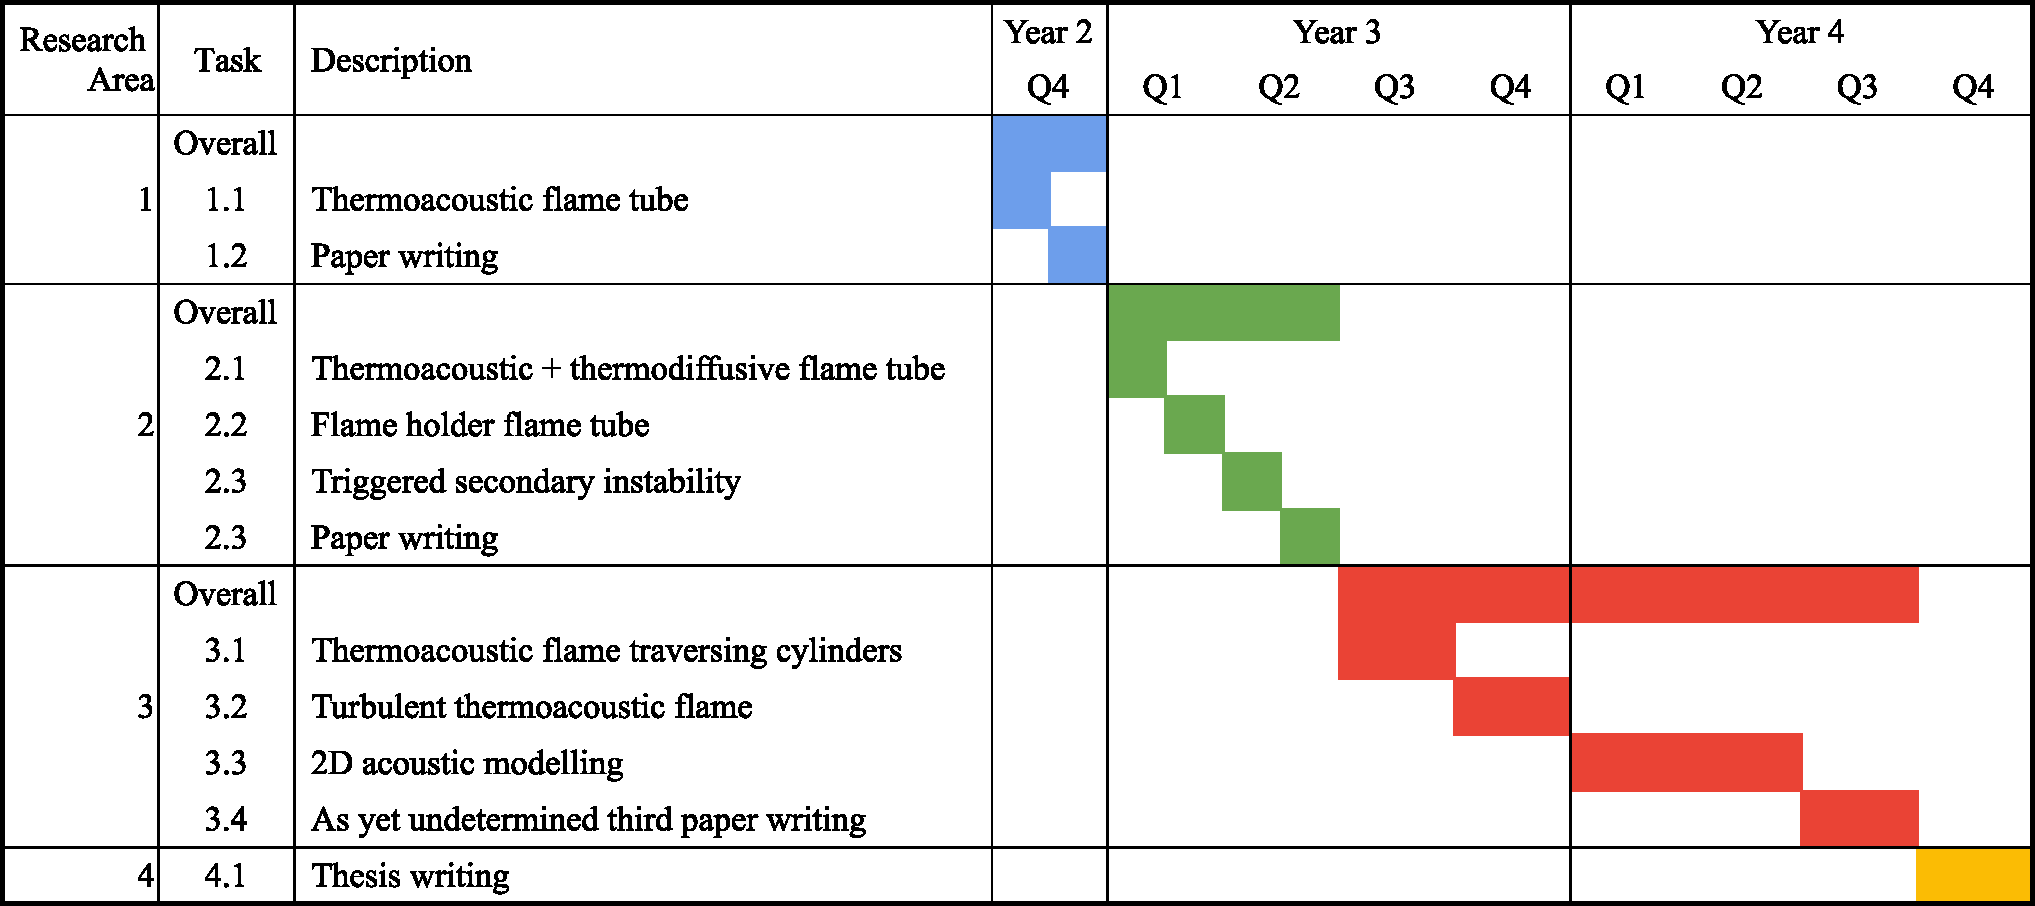
\includegraphics[scale=0.5]{assets/graphs/2YR_Gantt.pdf}
\caption{Gantt chart organising tasks for the remaining seven quarters of my PhD.}
\label{fig:gantt}
\end{figure}

There are seven quarters left before my thesis must be written and submitted and the three and a half years of my PhD, beginning January 2024, are over. Currently, I am organising future work into the journal articles (papers) they fit into and timetabling these tasks accordingly:
\setlist[enumerate]{label={\arabic*.}}
\begin{enumerate}
\item \textbf{Paper 1. One quarter needed total.} This paper will focus on the ADCBC method, with examples of an acoustic bump, acoustic standing wave and thermoacoustic flame tube. The method will be explained alongside post-processing for the acoustic domain.
    \begin{enumerate}
    \item Completion of the simulation, post-processing and analysis of a thermoacoustic flame tube for a journal article has yet to be fully done. Primarily due to the analysis, which will be used for further thermoacoustic simulations, half a quarter is needed. Calculations of Rayleigh Indices, RI and acoustic envelopes need to be performed and the aforementioned interpolation issue needs to be investigated
    \item The rest of the quarter will be used to write the paper.
    \end{enumerate}
\item \textbf{Paper 2. Two quarters needed total.} This paper will focus on applications of the ADCBC method to simulations of various physical phenomena, each of which do not require large developments of the ADCBC method.
    \begin{enumerate}
    \item A thermodiffusive and thermoacoustically unstable flame require dynamic inflow non-acoustic velocities. Alongside simulations, post-processing and analysis I estimate this to take half a quarter.
    \item Similarly, a counterflow flame holder flame might require some extra work to implement the correct physical initial conditions for a simulation using ADCBC restarted from an unsteady simulation using non-reflecting NSCBC. I estimate this to take half a quarter too.
    \item The final phenomena is a simulated secondary thermoacoustic instability, which relies on the prior work to change inflow speeds dynamically and impose an additional acoustic field, as mentioned above. I estimate this to take half a quarter too.
    \item The rest of the two quarters will be used to write the paper.
    \end{enumerate}
\item \textbf{Potential third paper. Four quarters needed total.} This paper not yet in focus and its specific contents will be determined by the remaining time and feasibility of each individual task.
    \begin{enumerate}
    \item Simulation of a thermoacoustically unstable flame travelling through arrays of cylinders in a broader domain will likely take a quarter, since I may have to introduce a queue system for each boundary node and perform three-dimensional simulations.
    \item The aforementioned self-turbulent thermoacoustically unstable flame simulation also requires development of the ADCBC to be compliant with turbulent flows and is estimated to take a quarter.
    \item I suspect investigations into more elaborate acoustic modelling will be a deeper rabbit hole, which could take a long time if it is provided. By restricting the scope to what is reasonable to do in the rest of my PhD, I estimate it should only take one quarter.
    \item The rest of the four quarters will be used to write a paper from the resulting research.
    \end{enumerate}
\item \textbf{Thesis. Two quarters needed total.} This should be written in conjunction with the above to make the best use of time.
    \begin{enumerate}
    \item As mentioned, my thesis must be written by the end of 2027 and I estimate it will take roughly one quarter to put together alongside other work.
    \end{enumerate}
\end{enumerate}
This is organised into a Gantt chart in \fig{fig:gantt}, showing how the remaining nine quarters will be used in sequence. Further up-to-date details on this plan are given at \href{https://www.dropbox.com/scl/fi/4w62xppcfkywnr7nm8a6v/plan-Y3.md?rlkey=yx4ez0nmqjaabqseotnzfiqsn&st=lll313fe&dl=0}{\texttt{this link}}.


